\section{Phase separation}

To understand the formation of bijels, the difference between nucleation and growth and spinodal decomposition must be understood. These processes 
govern how distinct domains emerge and evolve within a binary mixture upon quenching into the two-phase region of the phase diagram. While nucleation and growth involve the formation 
and expansion of isolated domains, spinodal decomposition leads to the spontaneous, interconnected structuring characteristic of bijels. Investigating both mechanisms provides insight 
into how thermodynamic and kinetic pathways influence the resulting microstructure, and why spinodal decomposition is uniquely suited for producing the bicontinuous 
architecture essential to bijels. A schematic free energy and phase diagram is plotted in Figure \ref{fig:phase_diagram}

\begin{figure}
    \centering
    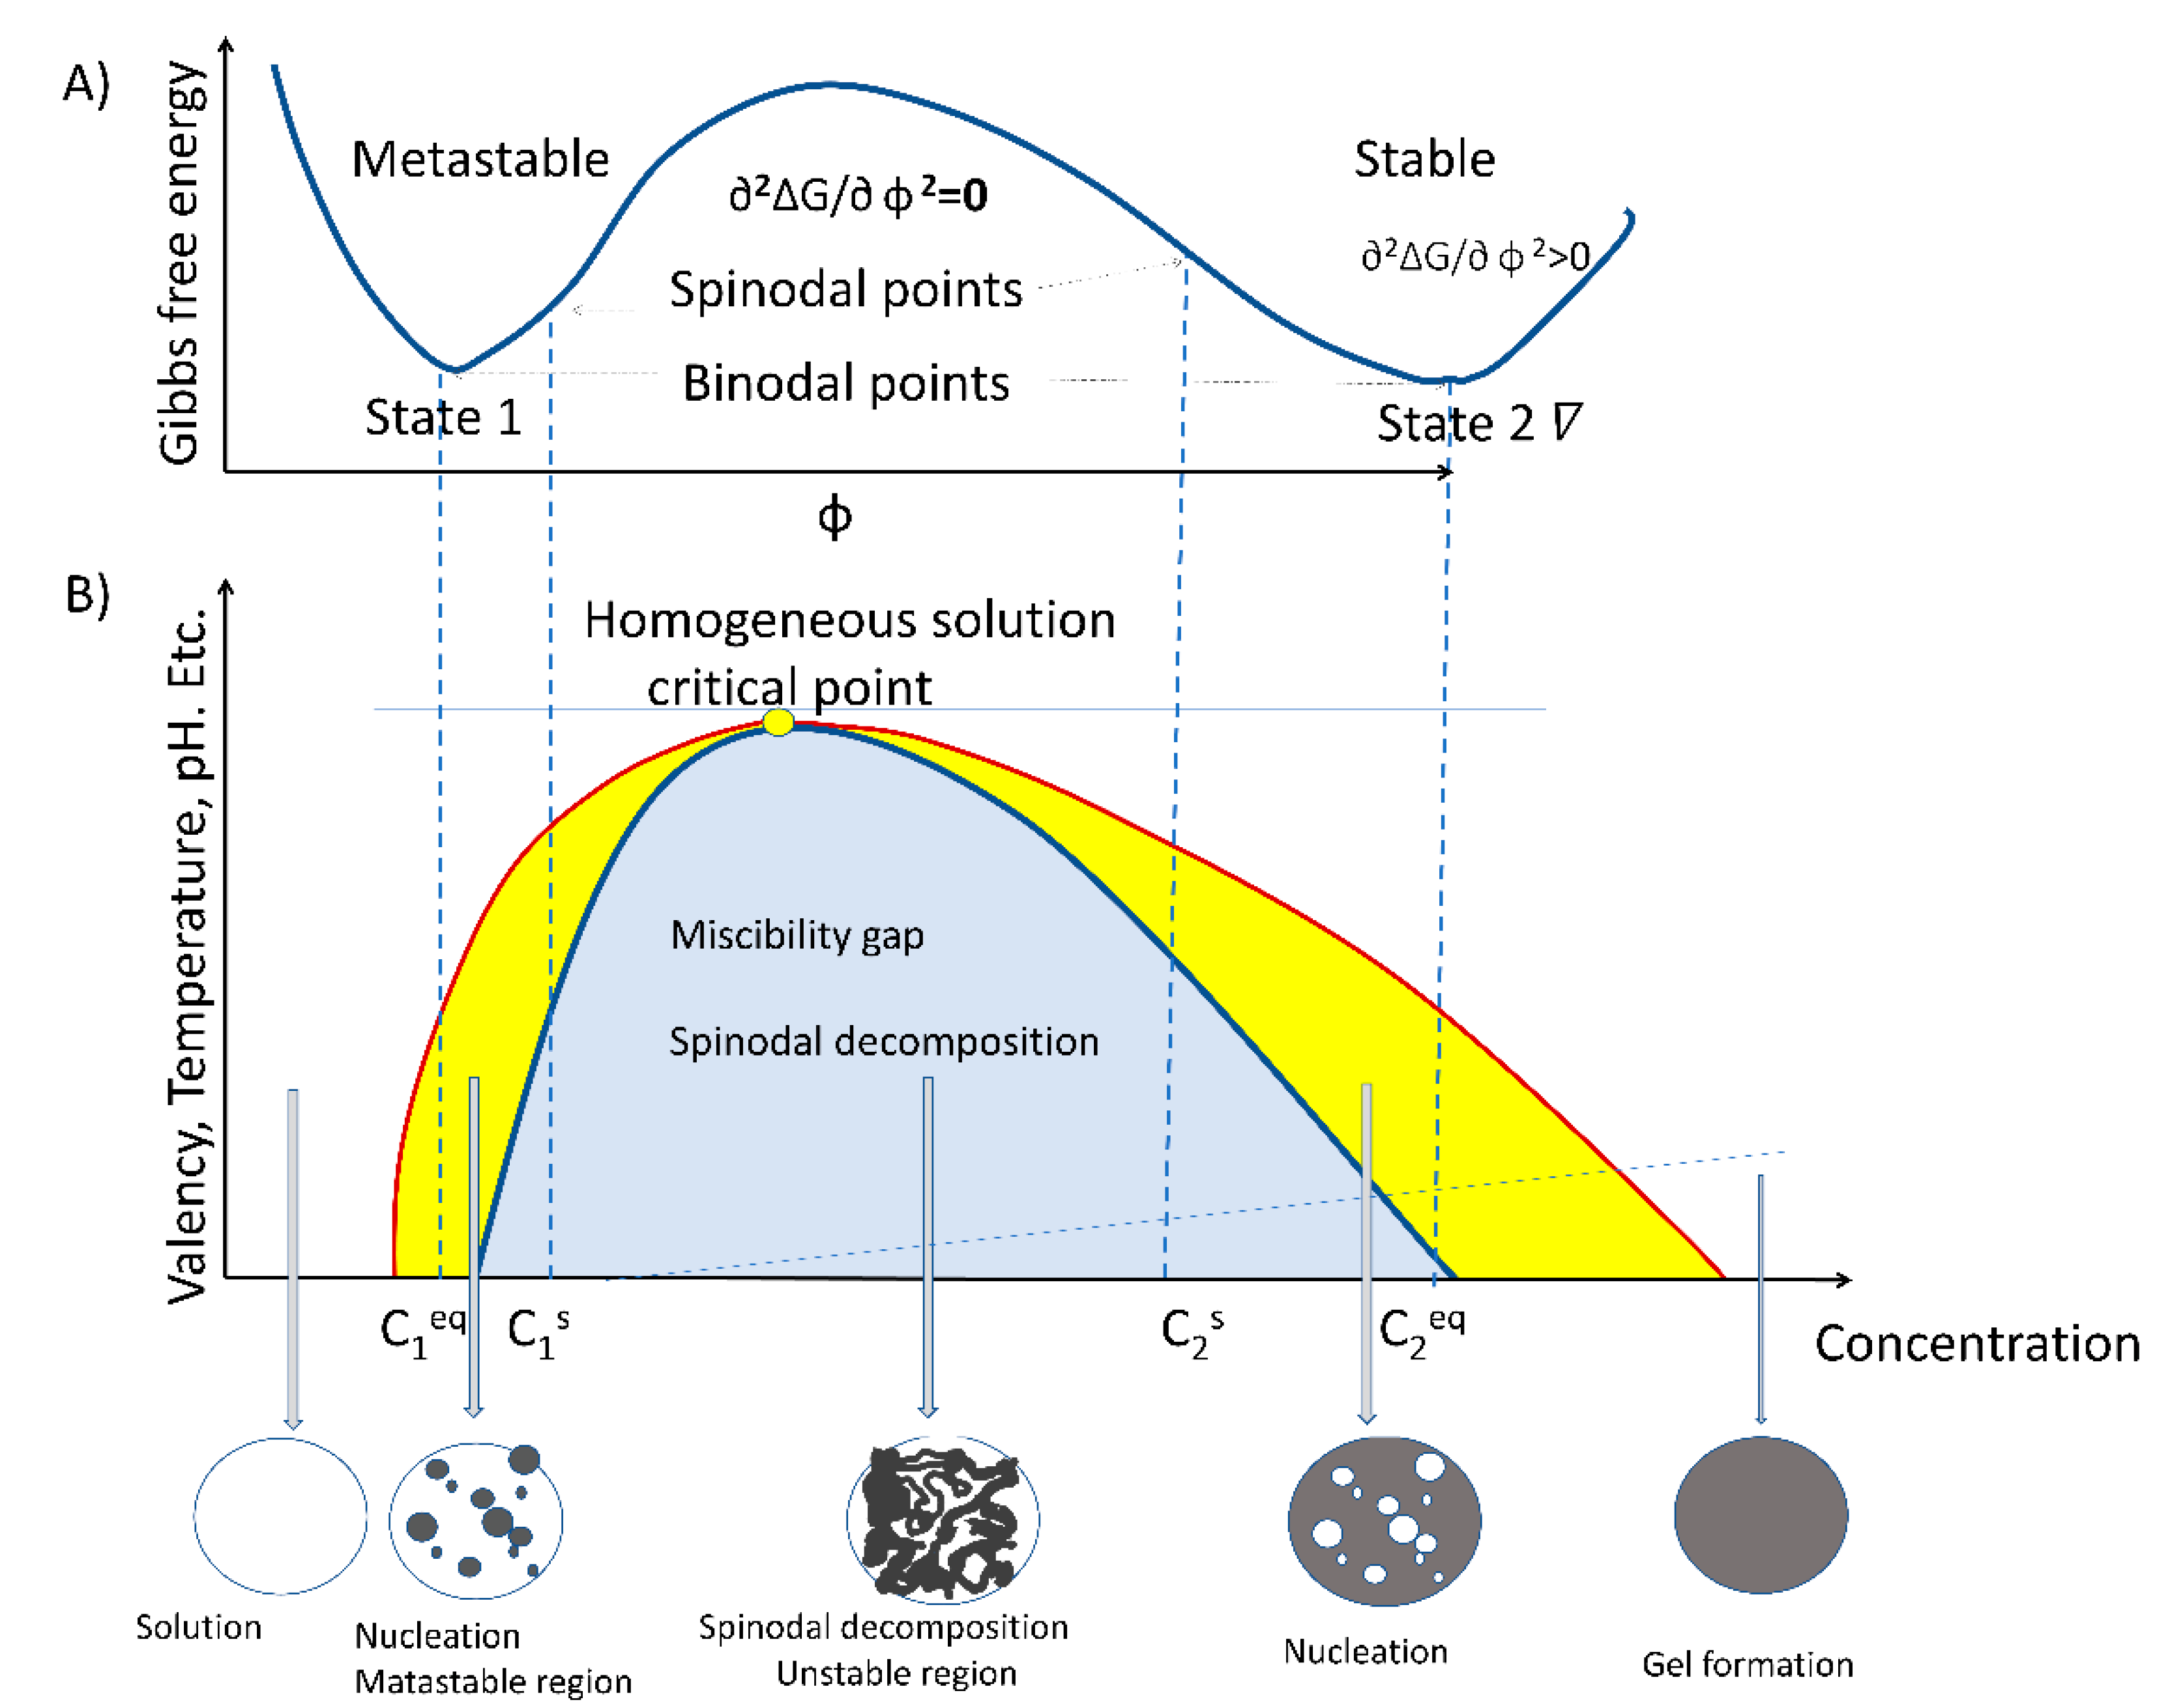
\includegraphics[scale = 0.7]{../figures/literature_review/phase_diagram.png}
    \caption{Schematic of a phase diagram obtained from a free energy curve demonstrating key features of the free energy landscape that correspond
             to the phase diagram. Reprinted Figure 1 from
             Guillen-Chable, F.; Bayona, A.; Rodríguez-Zapata, L. C.; Castano, E. Phase Separation of Intrinsically Disordered 
             Nucleolar Proteins Relate to Localization and Function. IJMS 2021, 22 (23), 13095. with permission under the Creative Common CC BY license.}
    \label{fig:phase_diagram}
\end{figure}

The thermodynamic equilibrium of a binary fluid mixture can be described by its Gibbs free energy, given as $G = \Delta H - T \Delta S$, where \(\Delta H\) is the enthalpy change, 
\(T\) is temperature, and \(\Delta S\) is the entropy change. The onset of phase separation occurs at the binodal line, defined where \(\frac{dG}{dx} = 0\), with \(x\) representing the composition. 
Although the system is metastable, it remains uniform until fluctuations give rise to small nuclei. The free energy of each nucleus reflects a 
balance between the bulk free energy gain from phase separation and the interfacial energy penalty, expressed as \(\Delta G = \frac{4}{3}\pi r^3 \Delta g_v + 4 \pi r^2 \sigma\), where \(r\) is 
the nucleus radius, \(\Delta g_v\) is the free energy change per unit volume, and \(\sigma\) is the interfacial tension \cite{thanh_mechanisms_2014}. 
Nuclei that exceed the critical radius \(r_c = \frac{2\sigma}{|\Delta g_v|}\) will grow, driving the system toward phase separation via nucleation and growth \cite{thanh_mechanisms_2014}. 
This transformation process is commonly modeled by the Avrami equation, \(Y = 1 - \exp(-K t^n)\), where \(Y\) is the 
transformed fraction, \(K\) is a rate constant incorporating nucleation and growth kinetics, and \(n\) is the Avrami exponent, which reflects the dimensionality and mechanism of the transformation
\cite{avrami_kinetics_1939}.

At the binodal, the system is still metastable, meaning that unless perturbations are introduced to form nuclei, the mixture remains homogeneous \cite{thanh_mechanisms_2014}.
However, a deeper quench into the two-phase region leads to the spinodal line, defined by the stability criterion \(\frac{d^2G}{dx^2} = 0\) \cite{cahn_free_1958}. 
Within this region, the system is unstable to even infinitesimal composition fluctuations, and phase 
separation proceeds spontaneously without the need for nucleation. This process, known as spinodal decomposition, is characterized by the continuous and simultaneous growth of interconnected 
domains of both phases \cite{cahn_free_1958}. Unlike nucleation and growth, which relies on localized events, spinodal decomposition 
results in a bicontinuous structure driven by the system's attempt to minimize 
free energy through composition modulation \cite{cahn_free_1958}. The dynamics of spinodal decomposition were characterized by Cahn and Hilliard \cite{cahn_spinodal_1961}. 
We first begin by defining the free energy of a regular solution, known as the bulk free energy given by

\begin{equation}
    G_m (c) = \chi (1 - c)c + N_a k_B T \left[(1 - c)\ln(1 - c) + c \ln(c)\right]
\end{equation}

This bulk free energy characterizes the thermodynamic driving forces for phase separation. Alternative forms, such as the Landau-Ginzburg or Flory-Huggins models, may also be used depending on system 
specifics. In real systems, the interface between two partially miscible fluids is not sharp, meaning that the composition transitions smoothly across a finite interface width. To account for this, a 
gradient energy penalty is added to the free energy functional, penalizing sharp spatial variations in composition. The total free energy functional is written as

\begin{equation}
    F[c] = \int \left( f(c) + \frac{\kappa}{2}|\nabla c|^2 \right) \, dV
\end{equation}

where $\kappa$ is the gradient energy coefficient controlling the interface width. Larger \(\kappa\) values correspond to wider interfaces.
The chemical potential is then defined as the variational derivative of the free energy functional,

\begin{equation}
    \mu = \frac{\delta F}{\delta c} = \frac{df}{dc} - \kappa \nabla^2 c
\end{equation}

This chemical potential enters the mass flux expression via a Fickian transport law,

\begin{equation}
    \vec{J} = -M \nabla \mu
\end{equation}

where $M$ is the mobility and could potentially be a function of $c$. Assuming no advection and applying mass conservation for the order parameter, we obtain,

\begin{equation}
    \frac{\partial c}{\partial t} = -\nabla \cdot \vec{J}
\end{equation}

Substituting in the expression for \(\vec{J}\) leads to the Cahn-Hilliard equation 18 in reference \cite{cahn_spinodal_1961},

\begin{equation}
    \frac{\partial c}{\partial t} = \nabla \cdot \left( M \nabla \mu \right)
\end{equation}

This equation describes the diffusive evolution of the conserved field $c$ during phase separation. It captures the system's tendency to minimize its total free energy 
by redistributing the order parameter according to gradients in chemical potential. The Cahn-Hilliard framework naturally incorporates interfacial tension and allows for smooth, 
continuous transitions between phases, making it highly suitable for modeling non-ideal mixing in systems such as bijels.

The most important difference between these two phase separation methods is the morphology of the phase separated structure. While nucleation and growth generates discontinuous droplets,
spinodal decomposition creates continuous domains that have tunable domain sizes and tortuosity which are attractive in many materials applications such as battery electrodes, filtration
membranes and catalyst supports.

\section{Solid particles at fluid interfaces}

When micron sized particles are adsorbed by interfaces the attachment energy is large enough that they can become irreversibly trapped at fluid-fluid interfaces \cite{ngai_particle-stabilized_2015}. 
Once adsorbed, these 
particles reduce interfacial tension and act as physical barriers that prevent the coalescence of droplets, thereby making them highly effective emulsion stabilizers. Unlike molecular surfactants, 
which are dynamic and can desorb under certain conditions, colloidal particles remain adsorbed at the interface due to the significant energy required to detach them \cite{ngai_particle-stabilized_2015}. 
This mechanism 
is especially useful in systems such as Pickering emulsions, where the interfacial coverage and wettability of the particles determine the type and stability of the emulsion formed 
\cite{ngai_particle-stabilized_2015,velankar_non-equilibrium_2015}.
As such, understanding particle behavior at interfaces is essential for controlling the structure and longevity of particle-stabilized systems \cite{ngai_particle-stabilized_2015}. 
For particles that are smooth and simple and at an interface of oil and water, the attachment energy at the fluid interface can be calculated the Pieranski model, 
$G_{ads} = \sigma A_{rm} (1 - \cos{\theta_c})^2$, where $G_{ads}$ is the free energy reduction upon particle adsorption, $\sigma$ is the surface tension between the two 
fluids, and $\theta_c$ is the contact angle of the stabilizing particle. A schematic of a particle adsorbing at an interface is shown in Figure \ref{fig:pieranski_model},

\begin{figure}
    \centering
    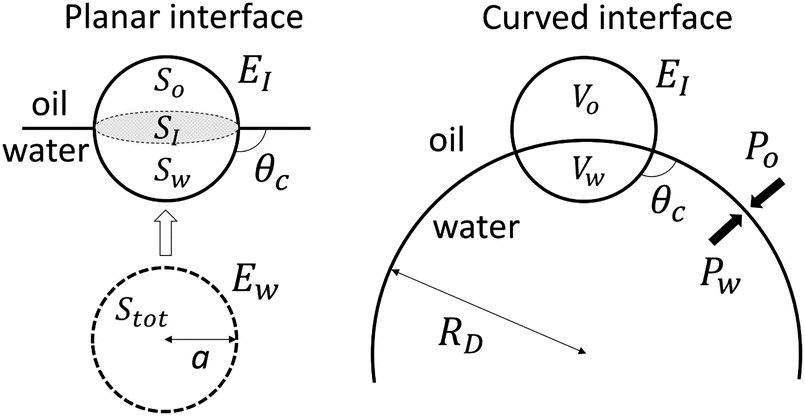
\includegraphics[scale = 0.5]{../figures/literature_review/particle_at_interface.png }
    \caption{Particle schematic at an interface demonstrating the various quantities of interest. Reprinted Figure 2.1 from
             Particle-Stabilized Emulsions and Colloids: Formation and Applications; Ngai, T., Bon, S. A. F., Eds.; RSC soft matter series; 
             with permission Royal Society of Chemistry, RSC Publishing Cambridge, 2015 under license number 1597404-1}
    \label{fig:pieranski_model}
\end{figure}

To obtain the Pieranski model, an energy balance between the interactions between the interface and the fluid phases can be written. The energy of the system before and after particle adsorption is 
different and can be characterized for the particle moving from water into the interface as,

\begin{equation}
    \Delta E_{IW} = E_I - E_w
\end{equation}

Where $\Delta E_{I}$ is the energy of the system when the particle is in the interface and $\Delta E_W$ is the energy of the system when the particle is completely in the water phase.
We define $\Delta E_{I}$ as

\begin{equation}
    E_I = A_w \sigma_{pw} + A_o\sigma_{po} + A_{I_1}\sigma_{ow} + V_w P_w + V_o P_o
\end{equation}

Where subscripts $w$, $o$ and $I$ represents the water phase, oil phase and interface respectively. $A_w$ and $A_o$ are the surface areas of the particle in the water and oil phases 
respectively, $V_w$ and $V_o$ are the volumes of water and oil phases respectively, $P_w$ and $P_o$ are the pressures of water and oil phases respectively. $A_{I_1}$ is the area of the 
interface with the particle. A similar equation can be written for the energy of the water phase, $E_w$

\begin{equation}
    E_w = (A_w + A_o)\sigma_{pw} + A_{I_2}\sigma_{ow} + (V_w + V_o)P_w
\end{equation}

$A_{I_2}$ is the area of the interface without the particle. The change in the interface energy upon adsorption of the particle can be computed to obtain

\begin{equation}
    \Delta E_{IW} = A_o(\sigma_{po} - \sigma_{pw}) - A_p\sigma_{ow} + V_o(P_o - P_w)
\end{equation}

A similar construction can be done for the oil phase to obtain 

\begin{equation}
    % \Delta E_{IO} = -\sigma_{ow}(A_w\cos{\theta_c} + A_p - \frac{2 V_o}{R_d})
    \Delta E_{IO} = A_w(\sigma_{pw} - \sigma_{po}) + A_p\sigma_{ow} - V_o(P_o - P_w)
\end{equation}

We now use the Young-Dupre equation relating the surface tensions of each component to one another, $\cos{\theta_c} = \frac{\sigma_{po} - \sigma_{pw}}{\sigma_{ow}}$ and the
Young-Laplace equation for a sphere, relating the pressure difference inside and outside a droplet $\Delta P$ to the radius of the droplet $R_d$, $\Delta P = \frac{2\sigma}{R_d}$
Substutions for $\sigma_{pw} - \sigma_{po}$ and $P_o - P_w$ are made, resulting in 

\begin{equation}
    \begin{split}
        \Delta E_{IW} &= \sigma_{ow}(A_o\cos{\theta_c} - A_p - \frac{2 V_o}{R_d}) \\
        \Delta E_{IO} &= -\sigma_{ow}(A_w\cos{\theta_c} + A_p - \frac{2 V_o}{R_d})
    \end{split}
\end{equation}

From this the Pieranski model, the adsorption energy can be seen to depend on the contact angle, surface tension and contact area of the particles. This indicates that larger, neutrally wetting
particles adsorbing onto interfaces with high surface tension have a high driving force for adsorption. \cite{ngai_particle-stabilized_2015,reeves_particle-size_2015} This adsorption process 
can be orders of magnitude larger than the thermal energy of the system, calculated as $k_b T$ where $T$ is the temperature of the system and $k_b$ is the Boltzmann constant. This results in 
irreversible adsorption of particles at interfaces. \cite{binks_pickering_2001}

In addition to the adsorption of particles on the interface, the contact angle of the particles determine the dispersed phase of an emulsion and its microstructure. \cite{velankar_non-equilibrium_2015}
Hydrophillic particles tend to prefer to form oil in water emulsions while hydrophobic particles prefer to form water in oil emulsions. \cite{ngai_particle-stabilized_2015}
This occurs as the particles preferentially wet one phase over another, causing the interface to bend as the emulsion forms. Neutrally wetting particles are preferred in the formation of 
bijels as no preferential curvature is imparted onto the bijels, fulfilling one of the requirements of a minimal surface in that the mean curvature must be zero. \cite{jinnai_interfacial_2001}

\section{Anisotropic particles}

As the library of available particle shapes continues to grow, it becomes increasingly important to understand how these anisotropic particles behave at fluid interfaces
\cite{wu_recent_2016, cavallaro_curvature-driven_2011}.
Unlike spherical particles, anisotropic particles introduce directional interactions and complex rotational dynamics which can significantly 
influence interfacial assembly and emulsion stability \cite{read_dimerization_2020, davies_dipolar_2015,morgan_understanding_2013}. 
Their shape can dictate not only their orientation at the interface but also how they interact, and jam, 
ultimately affecting the structure and mechanical properties of the resulting material \cite{hijnen_bijels_2015}.
This is relevant for systems like bijels, where the precise arrangement of particles at the interface affects how the bijel jams in place, generating new timescales or 
capillary bridging not characterized in bijels made with spheres \cite{gunther_timescales_2014,hijnen_bijels_2015,witt_bijel_2013}.

Anisotropic particles exhibit shape-dependent interfacial behavior due to their ability to induce complex multipolar capillary interactions. When adsorbed at a fluid-fluid interface, these 
particles distort the surrounding interface in order to maintain a mean curvature of zero, in accordance with the Young-Laplace equation. This distortion creates curvature gradients around the 
particle that interact with nearby particles or features on the interface, giving rise to anisotropic capillary forces \cite{loudet_capillary_2005, cheng_shape-anisotropic_2013}. 
Computational simulations further support this complexity, showing that ellipsoidal particles can adopt a variety of metastable orientations 
depending on initial conditions and perturbations encountered during adsorption or rearrangement at the interface \cite{gunther_lattice_2013, newton_influence_2014}. 

\begin{figure}
    \centering
    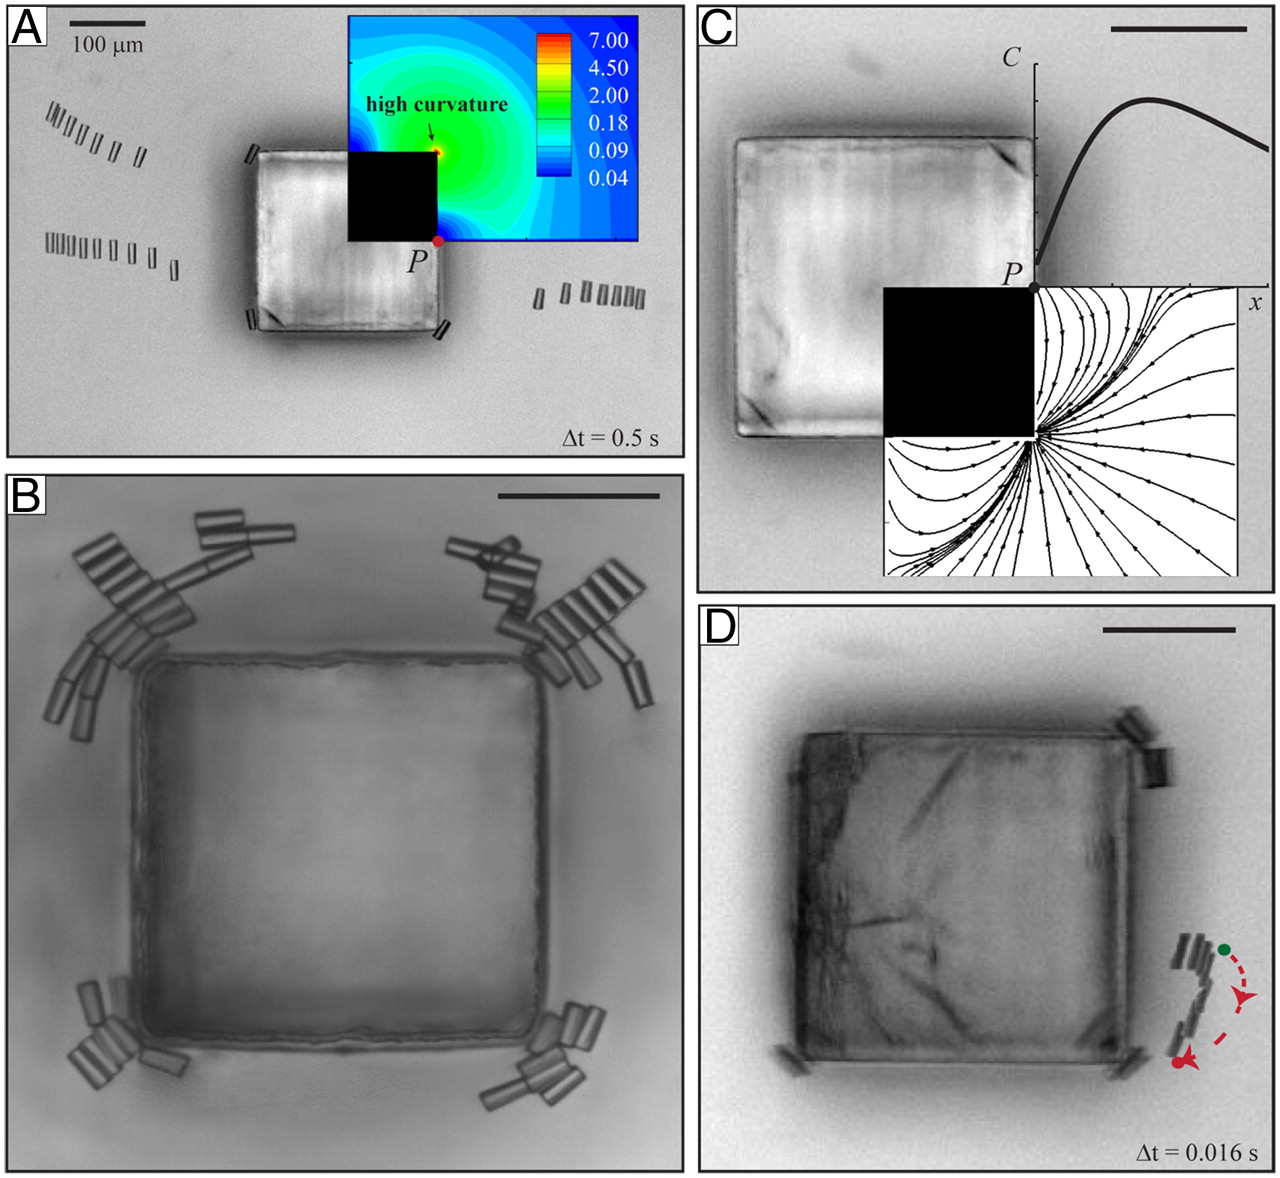
\includegraphics[scale = 0.3]{../figures/literature_review/curvature_driven_assembly.jpeg}
    \caption{Self assembly of particles at points of large curvature gradients. Reproduced from Figure 5 in Cavallaro, M.; Botto, L.; 
             Lewandowski, E. P.; Wang, M.; Stebe, K. J. Curvature-Driven Capillary Migration and Assembly of Rod-like Particles. 
             Proc. Natl. Acad. Sci. U.S.A. 2011, 108 (52), 20923-20928 under the CC-BY license}
    \label{fig:curvature_gradient}
\end{figure}

When looking at arrays of ellipsoidal particles at interfaces, curvature gradients control the dynamics of the system. Figure \ref{fig:curvature_gradient} illustrates the effect that
Cavallaro and co-workers identified. They showed how curvature gradients created at the edges of a 
square rod caused directed assembly of cylinders, with the driving force strong enough to overcome gravity \cite{cavallaro_curvature-driven_2011}. Other works have introduced how these features are 
particle shape dependent with greater control over the curvature gradient providing a means to control particle self assembly \cite{read_dimerization_2020, sharifi-mood_curvature_2015}.
Earlier work in the literature identified that ellipsoidal particles prefer to arrange side to side state while cylinders prefer to arrange tip to tip with the particle geometric smoothness playing 
a role in this preference \cite{botto_capillary_2012}. These differences in particle arrangement could open up new possibilities for tailoring interfacial assemblies and the subsequent differences 
in microstructure obtained in a bijel.

Ellipsoidal particles have been used as stabilizers in bijels, resulting in bijels that have smaller domains than those made with spherical particles at the same volume fraction. This was identified 
to arise from the greater surface area to volume ratio of ellipsoidal particles compared to spherical particles \cite{gunther_timescales_2014}. The evolution of the microstructure is also distinct 
to bijels stabilized with spheres, demonstrating two timescales at early and later timesteps \cite{gunther_timescales_2014}. The short timescale is during formation of the bijel, when particles 
are adsorbed onto the interface and rotate to align with the interface. At longer timescales, capillary interactions between particles lead to reordering of particles at the interface, leading 
to a different interfacial configuration and microstructure \cite{gunther_timescales_2014}. 

\begin{figure}
    \centering
    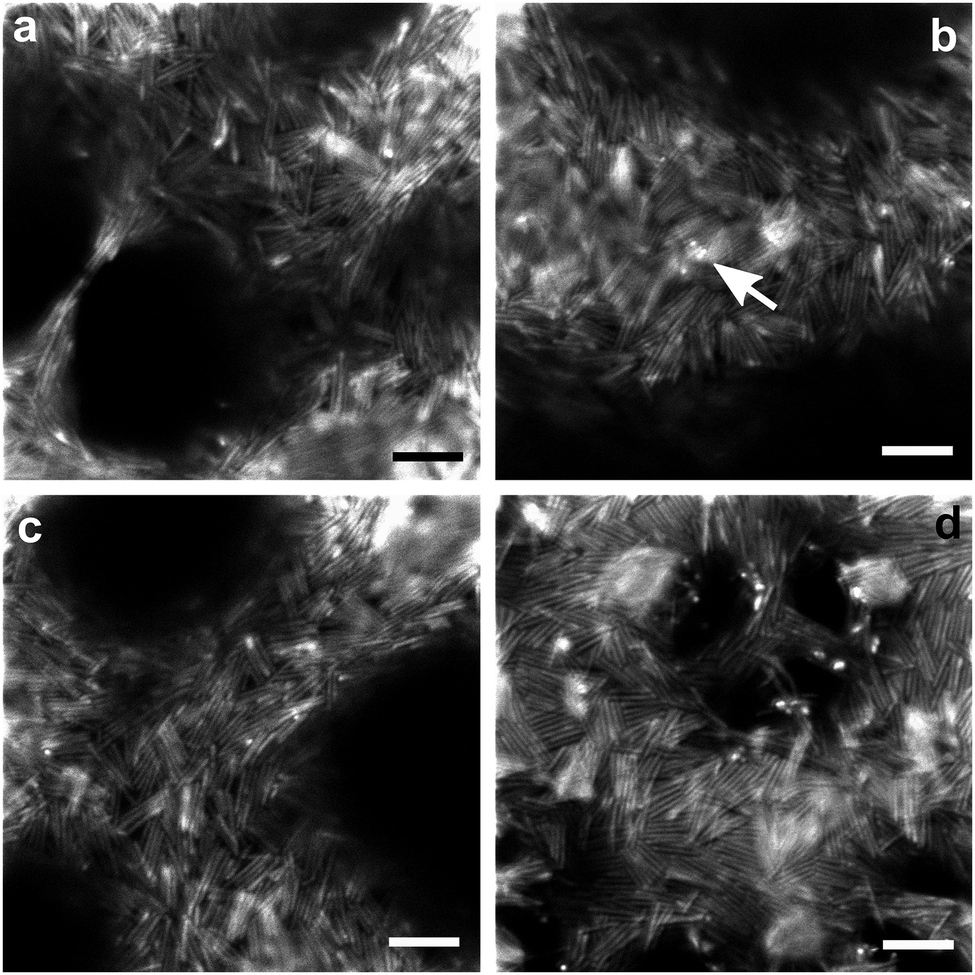
\includegraphics[scale = 0.3]{../figures/literature_review/rods_bijels.png}
    \caption{Bijels stabilized by rod like particles, demonstrating 'flippers' at the interface, which are particles that flip out of the interface due to stress from adjacent particles. 
             Reproduced from Figure 3 in Hijnen, N.; Cai, D.; Clegg, P. S. Bijels Stabilized Using Rod-like Particles. Soft Matter 2015, 11 (22), 4351-4355 under the CC-BY license}
    \label{fig:rod_bijel_flippers}
\end{figure}


Rod like particles have also been used as stabilizers in experiments, identifying that the length scale of the pores of the bijels follows $ L \propto \frac{1}{\phi_p} $ even if the 
proportionality constant is different. Figure \ref{fig:rod_bijel_flippers} demonstrates bijels stabilized by rod like particles showing that particles flip out of the interface due to steric 
forces from adjacent particles. This flipping can provide structural support between the domains, providing the bijel with greater mechanical stability.
While the proportionality constant depends on particle geometry, this trend has been observed across various particle shapes 
\cite{hijnen_bijels_2015, madivala_exploiting_2009, gunther_timescales_2014, daware_emulsions_2015, loudet_capillary_2005, cheng_shape-anisotropic_2013}. 

\section{Rheology}

Understanding the rheology of emulsions, particularly bijels, is essential because it directly impacts both their fabrication and practical use \cite{haase_situ_2016}.
Previous investigations have characterized that bijels are non-Newtonian fluids with a yield stress and shear thinning behavior \cite{macmillan_rheological_2019}.
A non-Newtonian fluid is one whose viscosity is not constant but varies with the applied shear rate or stress. In Newtonian fluids like water 
or air, there is a linear relationship between shear stress and shear rate, meaning viscosity remains the same regardless of how fast the fluid is sheared \cite{mezger_rheology_2020}. 
Non-Newtonian fluids, on the other hand, deviate from this behavior and may exhibit shear thinning, shear thickening, yield behavior or viscoelasticity with no fluid constrained to one behavior
\cite{mezger_rheology_2020}. Shear thinning and thickening here define that the viscosity increases at a slower and more rapid rate than the applied shear rate., while yield behavior implies that 
the viscosity is non-zero when no shear is applied \cite{mezger_rheology_2020}. Viscoelasticity appears when the shear response of the fluid is dependent upon the frequency of the applied shear, 
indicating that the fluid has both liquid and solid like characteristics \cite{mezger_rheology_2020}. These properties often appear in soft matter and multiphase systems where microstructure and 
particle interactions influence flow behavior.

\begin{figure}
    \centering
    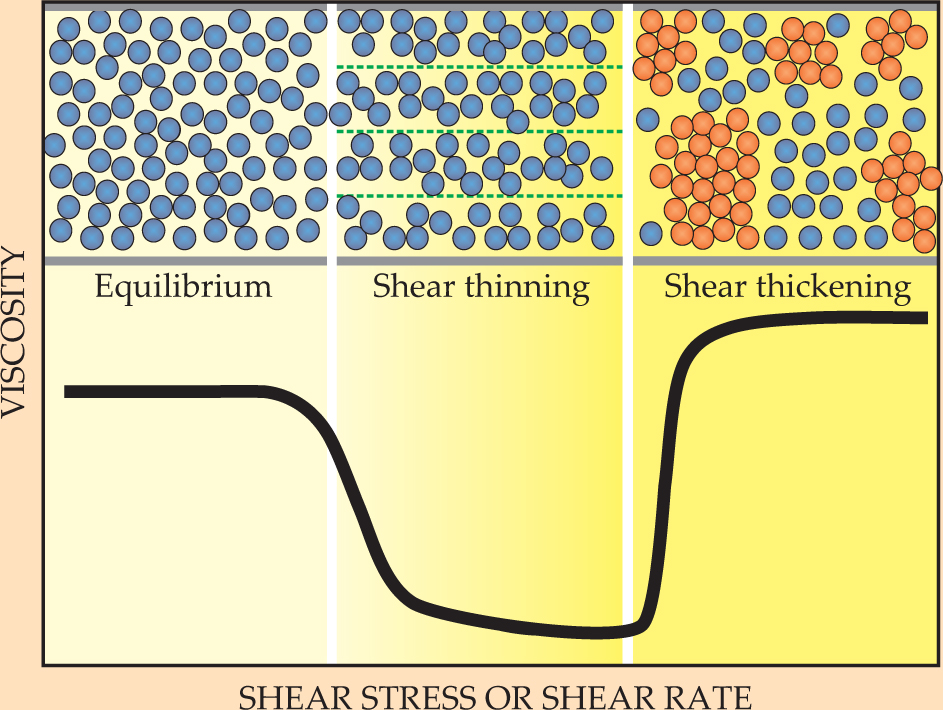
\includegraphics[scale = 0.3]{../figures/literature_review/shear_suspensions.jpeg}
    \caption{Schematic of suspensions under shear demonstrating shear banding and shear aggregates modifying the rheological properties of a suspension. 
             Reproduced from Figure 2 in Wagner, N. J.; Brady, J. F. Shear Thickening in Colloidal Dispersions. Physics Today 2009, 62 (10), 27-32 under the CC-BY license}
    \label{fig:suspension_shear}
\end{figure}

Suspensions and emulsions are examples of non-Newtonian fluids due to the presence of dispersed particles or droplets within a continuous phase
\cite{brader_nonlinear_2010, besseling_three-dimensional_2007, xu_relation_2013}.
In suspensions, the interaction  between solid particles—such as hydrodynamic forces, electrostatic repulsion, and steric hindrance—creates microstructural rearrangements under flow, leading to 
non-linear viscosity responses \cite{brader_nonlinear_2010, besseling_three-dimensional_2007}. Figure \ref{fig:suspension_shear} demonstrates the shear properties of an example suspension, 
demonstrating how shear thinning and shear thickening can occur in suspensions. At low shear, particles may aggregate or form a network that resists deformation, while higher shear rates can break 
down these structures, resulting in shear thinning. In dense systems, particles may experience contact-induced resistance or jamming, causing shear thickening \cite{brader_nonlinear_2010}. 

Emulsions behave similarly with droplet deformation, coalescence, and interactions 
among droplets generating time-dependent and non-linear responses to shear. When particles are used to stabilize emulsions (e.g., in Pickering emulsions), their rigidity 
adds further resistance to flow and deformation, contributing to complex, often viscoelastic, rheological behavior.
Madivala et al. showed that Pickering emulsions stabilized with rod-like particles had enhanced stability under shear, with greater resistance observed as particle aspect ratio increased 
\cite{madivala_exploiting_2009}. They identified this improvement to be due to improved interfacial coverage of ellipsoidal particles at interfaces and the enhanced elasticity of the interface,
allowing for the droplet to elongate more before failure. These improvements also extend to disc like particles with other investigations into the resistance to shear of emulsions stabilized by
graphene nanosheets, showing that they were able to provide better resistance to shear than spherical particles \cite{imperiali_simple_2014}. This was due to the graphene nanosheets overlapping one
another during shear, creating greater resistance to the applied shear and a higher apparent viscosity. In this case too, the overlap of graphene nanosheets was shown to result in greater interfacial
elasticity inferred through surface tension measurements of droplets with graphene stabilizers \cite{sun_assembly_2013}.

\begin{figure}
    \centering
    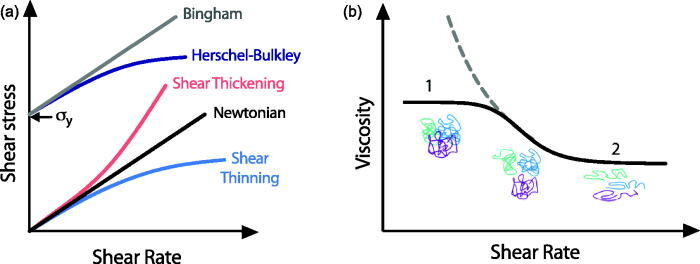
\includegraphics[scale = 4]{../figures/literature_review/Flow-curves.png}
    \caption{Schematic of expected shear stress as a function of applied shear rate for various models of fluids on the left and a shear thinning material on the right, demonstrating
             the yield stress at low strain rate followed by shear thinning and the infinite shear rate plateau. Reproduced from Cooke, M. E.; Rosenzweig, D. H. The Rheology of Direct 
             and Suspended Extrusion Bioprinting. APL Bioengineering 2021, 5 (1), 011502 under the CC BY license.}
    \label{fig:shear_theory}
\end{figure}

Several theoretical models have been developed to describe the behavior of non-Newtonian fluids under constant shear. The schematic representation of these models is shown in
Figure \ref{fig:shear_theory}. The power law Model is commonly used to represent shear thinning or 
thickening, with the equation \(\sigma = k \dot{\gamma}^n\), where \(\sigma\) is shear stress, \(\dot{\gamma}\) is shear rate, \(k\) is the consistency index, and \(n\) is the flow index 
\cite{mezger_rheology_2020}.
For \(n<1\), the fluid is shear thinning and for \(n>1\), shear thickening \cite{mezger_rheology_2020}.
The Bingham plastic model and Herschel-Bulkley model account for yield stress, with the latter being more general by 
including power-law behavior after yielding, defined as $\sigma = \sigma_y + k \dot{\gamma}^n$ \cite{mezger_rheology_2020}.
Shear models that include viscoelasticity have also been developed such as the  Maxwell and Kelvin-Voigt 
models \cite{mezger_rheology_2020}.
They are used when the fluid exhibits both solid- and liquid-like characteristics under stress, incorporating time-dependent strain responses and relaxation phenomena. These models help 
predict and quantify the behavior of complex fluids in real-world applications \cite{mezger_rheology_2020}. 

Bicontinuous interfacially jammed emulsion gels (bijels) exhibit highly complex rheological behavior due to their unique microstructure. Bijels typically show yield stress and viscoelasticity, 
behaving like soft solids under low stress and flowing under high stress \cite{macmillan_rheological_2019, bai_dynamics_2015, lee_making_2013}.  The rigidity of the 
particle-laden interface resists deformation, until the applied shear rate is high enough to overcome the frictional contacts keeping particles in place \cite{boakye-ansah_controlling_2020}. 
Experimental studies have reported non-Newtonian behavior such as shear thinning, attributed to the gradual inability of the particles to resist shear \cite{macmillan_rheological_2019}.
Simulation studies using Lattice Boltzman have identified the failure mechanism of bijels stabilized by spherical particles to be due to shear induced ordering to the applied field before
particle ejection from the interface, causing domain coalescence \cite{bonaccorso_shear_2020}. However, the rheology of bijels is still an emerging field, 
with ongoing work focused on understanding how particle properties such as shape, particle size and contact angle affect flow behavior. One important find was that bijels were 
2D colloidal glasses percolating in 3D \cite{ching_bijel_2022}. 

Magnetic fields introduce a means of dynamically tuning the rheology of emulsions stabilized by magnetically responsive particles \cite{qiao_magnetorheological_2012}. 
In Pickering emulsions, magnetic fields can induce droplet deformation and change the rigidity of the particle monolayer, thereby changing the flow behavior \cite{qiao_magnetorheological_2012}. 
For bijels incorporating magnetic particles, external fields can affect the stability and elasticity of the interfacial particle layer or cause domain reorganization. These effects can lead to 
tunable yield stress, viscosity, and viscoelastic properties.

\section{Emulsion studies using Lattice Boltzmann}

Understanding the complex interplay between fluid phases and particles in emulsions requires modeling approaches that can capture hydrodynamic interactions, interfacial tension, and particle 
behavior at mesoscopic scales. The multicomponent Lattice Boltzmann method has emerged as a powerful tool for simulating such systems, as it bridges the gap between continuum fluid dynamics 
and molecular-level detail. LB models can naturally incorporate smooth interfaces, phase separation dynamics, and solid-fluid coupling, making them particularly well-suited for studying 
emulsion formation, coarsening, and stabilization mechanisms. This has enabled detailed investigations into how particle properties and flow conditions influence emulsion structure and rheology.

One significant contribution of LB simulations to emulsion research has been the study of dynamical scaling during spinodal decomposition, characterized as the growth of the lengthscale
over time following a power law behavior \cite{siggia_late_1979, furukawa_role_1994}. From the multicomponent Navier Stokes equation, Reynolds number dependent scaling exponents for the 
lengthscale of the system were identified that were termed the viscous limit, where the Reynolds number was low, and the inertial limit, where the Reynolds number is high \cite{kendon_inertial_2001}.
Multicomponent LB studies definitively demonstrated the ranges of Reynolds number where these scaling laws held and identified a broad crossover region \cite{kendon_inertial_2001, kendon_3d_1999}.

Additionally, the bijel itself was first realized computationally using LB simulations. \cite{stratford_colloidal_2005} A multicomponent LB model with neutrally wetting colloids based on the 
implementation by Ladd showed that coarsening interfaces could catch particles irreversibly adsorbing them and arresting coarsening once the interfacial area matched the cross sectional area of 
particles adsorbed \cite{stratford_colloidal_2005,ladd_numerical_1994}. The simulations also showed that these structures were stable over long periods of time, motivating and guiding the 
experimental realization of bijels in 2007 \cite{herzig_bicontinuous_2007}. These simulations provided an explanation of the dynamics and mechanistic reasoning behind the formation of bijels, 
allowing for the prediction of the microstructure. More recent LB studies have extended these findings by identifying the volume fraction and wetting angle needed to form bijels as opposed to 
Pickering emulsions \cite{jansen_bijels_2011}. The effect of the surface tension, fluid density and volume fraction of particles were also studied, showing that surface tension and fluid density 
had little effect on the microstructure of bijels and that the length scale of the bijel was inversely proportional to the volume fraction of particles \cite{jansen_bijels_2011}.

More recent LB studies by Gunther et al. have extended these findings by incorporating nonspherical particles, such as ellipsoids or rods, to explore how anisotropy influences interfacial behavior 
and emulsion morphology \cite{gunther_timescales_2014}. These particles introduce directional capillary interactions and exhibit preferred orientations at the interface, which can lead to enhanced 
jamming and altered domain stabilization with timescales of domain size change not observed with spherical particles arising from steric force driven particle reorientation. The orientation of 
ellipsoidal particles at interfaces was also characterized using a multicomponent LB, demonstrating the adsorption of ellipsoidal particles at interfaces could result in metastable orientations of 
particles \cite{gunther_lattice_2013}.

The LB method has also enabled exploration of external field effects, particularly magnetic fields acting on particles at interfaces. Simulations involving magnetic dipolar particles show that 
applying an external field can induce tilting, chaining, or reorientation of particles at the interface \cite{davies_interface_2014, davies_assembling_2014}. This effect was caused by interface 
deformation that caused dipolar or quadropolar capillary interactions. This was extended to analyzing the effect of Janus particles at interfaces of evaporating droplets that showed how they preferred 
to stick together on curved interfaces \cite{xie_direct_2017}.

These studies demonstrate the effectiveness of multicomponent LB methods in identifying and characterizing mesoscale phenomena relevant to soft matter systems. By capturing 
complex fluid-fluid and fluid-particle interactions, LB models provide a versatile platform for simulating emulsion dynamics, interfacial assembly, and 
microstructural evolution. From revealing the scaling laws of spinodal decomposition to enabling the computational discovery of bijels, LB simulations have offered valuable insights that would be 
difficult to obtain experimentally. Furthermore, the ability to incorporate anisotropic particles and external fields, such as magnetism, highlights the method's adaptability for exploring 
increasingly sophisticated and tunable systems. 

\section{Numerical modeling}

\subsection{Multiscale modeling algorithms}

A wide range of numerical methods exist for simulating the physics details in previous sections. The choice of method depends on the specific physical processes to be captured such as 
interface dynamics, hydrodynamic interactions, and thermal fluctuations—as well as computational efficiency and scalability. Below, we outline several commonly used approaches that have been 
applied in studies of complex fluids and soft matter systems.

The Volume of Fluid (VOF) method is a sharp-interface technique used to track the evolution of fluid-fluid interfaces within a fixed computational grid 
\cite{gopala_volume_2008, fleckenstein_volume-fluid-based_2015, deising_direct_2018}. In VOF, a scalar field representing the volume fraction of one 
fluid is defined for each grid cell to indicate the local phase composition. Interface reconstruction algorithms are then employed to geometrically 
localize the boundary between phases. The method is inherently mass-conserving and can handle large interface deformations, making it particularly 
effective for high-Reynolds-number flows and surface-tension-driven phenomena. However, VOF methods can struggle with accurately capturing interfacial 
curvature and are not well-suited for diffuse interfaces, which limits their applicability in modeling spinodal decomposition and phase separation 
processes such as those that form bijels.

Phase field methods use a diffuse-interface approach to model multiphase systems, representing fluid composition or phase identity through a continuous 
order parameter field governed by equations such as the Cahn-Hilliard or Allen-Cahn equations 
\cite{mendoza_evolution_2006, carmack_tuning_2018, chan_channel_2012}. These methods naturally capture smooth transitions between phases, enable
accurate computation of interfacial forces, and handle topological changes like coalescence and breakup with ease. Derived from variational principles, 
phase field models are thermodynamically consistent, making them particularly well-suited for simulating spinodal decomposition, wetting phenomena, and 
interfacial dynamics. However, their main limitations include the need for fine spatial resolution near interfaces to maintain accuracy and the relatively 
high computational cost of solving fourth-order PDEs, especially when coupled with full hydrodynamic models.

Brownian dynamics is a particle-based simulation method used to model the stochastic motion of colloidal particles suspended in a fluid 
\cite{huber_brownian_2019, yip_brownian_2005, elsawy_utility_2025}. It approximates the over-damped limit of Langevin dynamics by integrating 
particle trajectories under the influence of both deterministic forces—such as interparticle potentials or external fields—and random thermal 
forces representing collisions with solvent molecules. Hydrodynamic interactions may be included through approximate mobility tensors or omitted 
entirely, depending on the desired level of fidelity. Brownian dynamics is particularly well-suited for studying self-assembly, aggregation, and 
diffusion in dilute suspensions, where particle motion is dominated by thermal fluctuations. However, it does not model the surrounding fluid 
explicitly, limiting its ability to capture bulk fluid flow or interface-mediated interactions. As a result, Brownian dynamics is not sufficient 
on its own for simulating the coupled fluid-particle dynamics involved in bijel formation.

The Lattice Boltzmann Method (LBM) is a discretization of the Boltzmann equation of motion for molecules. \cite{qian_lattice_1992, succi_lattice_2018, shan_multicomponent_1995, swift_lattice_1996}
Unlike traditional CFD techniques such as phase field or VOF methods, LBM tracks the evolution of a 
particle distribution function within grid cells evolved through a discretized Boltzmann equation of motion. Macroscopic variables such as fluid density and 
velocity are recovered from the particle distributions through appropriate moment integration, and the Navier Stokes equation at the incompressible limit can be 
obtained through a Chapman-Enskog expansion of the LBM. \cite{qian_lattice_1992} The LBM has become an attractive tool for meso-scale CFD simulations due to its ease of algorithm 
implementation, highly parallelizable nature and ease of boundary condition implementation, allowing coupling to other physically relevant systems such as 
particles with varieties of potentials, external fields and deformable bodies. Importantly, LBM can be extended to handle multiphase and multicomponent fluids, using either color-gradient models, free energy formulations, 
or pseudopotential approaches to model non-ideal mixing. It also couples well to particle dynamics through momentum exchange schemes, making it a powerful framework for 
simulating colloidal suspensions, interfacial phenomena, and structurally complex systems like bijels. Its ability to capture both hydrodynamics and mesoscale thermodynamic 
behavior makes it particularly suited for the multi-scale requirements of stimuli-responsive emulsions.

In summary, the Volume of Fluid method offers robust interface tracking and mass conservation but lacks the ability to naturally capture interfacial curvature. 
Phase field methods provide thermodynamically consistent, diffuse-interface models ideal for phase separation, though they require fine resolution and are computationally intensive. 
Brownian dynamics excels at modeling particle-level stochastic motion but cannot resolve bulk fluid dynamics or interface evolution on its own. In contrast, the Lattice Boltzmann Method 
combines the strengths of mesoscopic fluid modeling with efficient handling of complex interfaces and straightforward coupling to particle dynamics. Its balance between computational 
efficiency, scalability, and physical fidelity across multiple scales makes LBM the most suitable method for simulating the rich interplay of hydrodynamics, phase separation, and particle 
interactions in stimuli-responsive emulsions such as bijels.

\subsection{Multicomponent models in the Lattice Boltzmann Method}

Several techniques exist in the lattice Boltzmann literature for modeling multicomponent or multiphase systems. These are the Shan-Chen (SC) 
pseudopotential model, the free energy (FE) model, the color gradient (CG) model, and the interface tracking (IT) model.
These methods differ fundamentally in their formulation and implementation, each offering unique advantages and trade-offs in terms of accuracy, 
stability, physical realism, and computational cost. Below, each approach is briefly reviewed, followed by a comparative discussion of their 
suitability for modeling stimuli-responsive emulsions such as bijels.

The SC model introduces fluid-fluid interactions via a local, density-dependent force, enabling spontaneous phase separation and interface 
formation without requiring explicit interface tracking. 
\cite{shan_lattice_1993, shan_simulation_1994, shan_multicomponent_1995, jansen_bijels_2011,gunther_timescales_2014}
Its simplicity and computational efficiency have made it a widely used method. However,
in this formulation, surface tension is not an independently controllable parameter. An effective mass defined from the density of each component
in each lattice point is used in the force calculation, meaning that it indirectly determines the surface tension in addition to the interaction
strength parameter.

The FE model is derived from a square-gradient free energy functional, which modifies the equilibrium distribution to incorporate thermodynamic 
forces driving phase separation. \cite{swift_lattice_1996, kendon_inertial_2001, briant_lattice_2004} Like the SC model, it naturally produces interfaces and captures interfacial tension. Unlike the SC model, however, 
the FE model allows for explicit control of surface tension and interface thickness via the bulk free energy parameters. This thermodynamic 
consistency makes it attractive for modeling systems with diffuse interfaces. The thermodynamics of the system can also be modified through changing the free energy used.
\cite{swift_lattice_1996, briant_lattice_2004, kendon_inertial_2001}
A key limitation, however, is its difficulty handling fluids with high density ratios, which can reduce its applicability in more extreme multiphase scenarios.

The CG model assigns color labels to each fluid component and applies a recoloring step to enforce immiscibility and sharpen the interface 
between fluids. 
\cite{mora_optimal_2021, latva-kokko_static_2005, huang_study_2014, liu_multiphase_2016}
This recoloring step is responsible for generating interfacial tension and enables precise control over interfacial properties such 
as surface tension and width. The model has demonstrated success in soft matter systems where interfacial control is critical. However, implementing 
the recoloring algorithm introduces additional complexity and requires careful parameter tuning to ensure stability and numerical consistency. \cite{mora_optimal_2021}

The IT model employs level-set or front-tracking techniques to explicitly track the location of fluid interfaces by evolving a separate indicator 
function, commonly defined using a level set technique, alongside the LB solver. \cite{haghani_hassan_abadi_conservative_2018, liang_lattice_2023}
This method achieves high accuracy in resolving interface position and curvature, making it ideal for problems 
involving surface tension-driven flows or sharp interfacial features. However, it is computationally intensive as the indicator function must be implemented alongside
the LB solver. 

Given these trade-offs, the Shan-Chen pseudopotential model is chosen for this research due to its balance between physical realism and computational 
efficiency. \cite{jansen_bijels_2011,gunther_timescales_2014, gunther_lattice_2013, xie_direct_2017}
Its ability to capture phase separation, interface formation, and emergent domain morphology without requiring explicit interface 
tracking or complex coupling makes it suitable for simulating the large-scale dynamics of bijels. Moreover, its straightforward coupling to 
colloidal particles facilitates the inclusion of particle-fluid and particle-interface interactions central to the system being studied.

\subsection{Particle dynamics}

In computational studies of particle-laden fluids, particles can be modeled either as point particles or as explicitly resolved rigid bodies. The choice between 
these approaches depends on the physical fidelity required, the computational cost, and the scales at which particle-fluid and particle-interface interactions must be resolved.

Point particle models treat colloids as infinitesimal entities that influence the surrounding fields through source terms or effective force laws. 
\cite{mehrabadi_direct_2018, prosperetti_point-particle_2007, frohlich_validation_2018}
In such models, particles do not occupy physical volume and their influence on the fluid is typically introduced via body forces or perturbations to the chemical potential field. 
This approach is computationally efficient and particularly useful for systems with a large number of particles or when only large-scale collective behavior is of interest. 
However, point particles cannot capture rotational dynamics, or hydrodynamic effects such as lubrication forces. Additionally, 
their interaction with phase interfaces is often prescribed rather than emergent, limiting their accuracy in systems like bijels where particles jam at fluid-fluid interfaces 
and significantly modify the interface topology.

In contrast, explicit particle models represent colloids as finite-size rigid bodies with well-defined shape, volume, and surface boundary conditions
\cite{ladd_numerical_1994, jansen_bijels_2011,gunther_timescales_2014}. These particles interact 
with the surrounding fluid through no-slip or slip boundary conditions, and their motion responds dynamically to hydrodynamic, capillary, and interparticle forces. By resolving 
particle geometry, these models allow for accurate representation of rotational motion, surface wetting and interfacial adsorption
\cite{jansen_bijels_2011, gunther_lattice_2013}.
This is important in bijel systems, where particle-induced jamming depend on particle shape, size, and surface wetting. 

An intermediate approach between point particles and explicitly resolved rigid bodies is the immersed boundary method (IBM), which represents extended particles as collections of 
point markers embedded in the fluid \cite{peskin_immersed_2002, luo_immersed-boundary_2008, spandan_parallel_2017}.
These markers interact with the fluid through momentum exchange that impose motion onto the surrounding fluid, effectively reconstructing 
the dynamics of a deformable or rigid object without requiring an explicit boundary mesh \cite{peskin_immersed_2002, luo_immersed-boundary_2008, spandan_parallel_2017}.
IBM has been widely used in biological and colloidal systems, to model the dynamics of deformable bodies \cite{peskin_immersed_2002, luo_immersed-boundary_2008, spandan_parallel_2017}.

For systems in which interfacial structure, jamming, or near-field hydrodynamics of rigid bodies play a central role as in bijel formation, explicit particle modeling 
is generally preferred as we are able to resolve the interfacial structure and near field hydrodynamics without the complications of IBM. This technique has been used in simulations of
bijels based on the Lattice Boltzmann Method and phase field techniques demonstrating its effectiveness in modeling
phenomena relevant to bijels \cite{jansen_bijels_2011,gunther_timescales_2014,carmack_tuning_2018}.

\subsection{Magnetic fields and particles}

% The Shan-Chen pseudopotential
% model is used to simulate the Cahn-Hilliard equation, defined below

% \begin{equation}
%     \begin{split}
%     \frac{\partial\phi}{\partial t}+\nabla\cdot\left(\phi\vec{u}\right) &= \nabla \cdot \left( \Gamma  \nabla\phi \right)
%     \end{split}
% \end{equation}

% where $c^k$, $M^k$ and $u^k$ is the concentration, mobility and velocity of species $k$ respectively while $\mu$ is the free energy of system. 
% \cite{shan_lattice_1993, shan_simulation_1994, he_lattice_1997, he_discrete_1998}



% A computational model designed to simulate soft matter systems 
% at the mesoscale must accurately represent both hydrodynamics and non-ideal mixing in order to capture the essential physics of emulsions, colloids, and phase-separating fluids. 
% A hydrodynamic model must be able to recover mass and momentum conservation of a incompressible fluid

% Modelling multicomponent dynamics requires incorporating a free energy model between fluids, allowing for the implementation of
% chemical potential driven mass transfer and surface tension. Typically this is done using a Cahn-Hilliard model based on a
% square gradient free energy functional. This captures the demixing characteristics of phase separating fluids and controls interface
% characteristics, providing surface tension and interface width characteristics. This model has been used in past investigations looking 
% into spinodal decomposition, domain growth and coarsening. 


% To fully capture mesoscale dynamics, the model must also resolve the coupling between hydrodynamic flow and composition gradients. This coupling 
% is essential for simulating phenomena such as Marangoni flows, interfacial instabilities, and anisotropic stress distributions that arise from 
% non-uniform compositions or curvature-dependent surface tension. Moreover, the model must support anisotropic or time-dependent external fields 
% (e.g., magnetic, electric, or shear) that influence mixing behavior. Computational frameworks that can evolve velocity, pressure, and composition 
% fields simultaneously—while ensuring thermodynamic consistency and mechanical stability—are critical for accurately describing the emergent structures 
% and transport properties in non-ideal soft matter systems.

% Given the multiscale modeling necessary to correctly simulate the physical system, one approach suggested to tackle this problem is the multicomponent
% Lattice Boltzmann Method. This technique bridges the length and time scales necessary in soft matter modeling through modeling the evolution of a particle
% distribution function. Hydrodynamic parameters are recovered through calculating the moments of the particle distribution function. One of the advantages of
% the Lattice Boltzmann Method its parallelize nature and ease of adding multiple physical phenomena. In the following sections, the implementation of the LBM
% and alternatives to the LBM will be presented.

% This work uses a multicomponent Lattice Boltzmann Method (LBM) to simulate the hydrodynamics of two partially miscible, 
% incompressible fluids as implemented in LB3D. The LBM solves the continuity and Navier-Stokes equation at low
% Mach and Reynolds numbers for the fluid, defined as, 

% \begin{equation}
%     \begin{split}
%     \frac{\partial\rho}{\partial t} + \nabla\cdot\left(\rho\vec{u}\right) &= 0 , \\
%     \frac{\partial\vec{u}}{\partial t} + (\vec{u}\cdot\nabla)\vec{u} &= - \frac{1}{\rho} \nabla p + \nu \nabla^2 \vec{u} ,
%     \end{split}
% \end{equation}

% incorporating density $(\rho)$, viscosity $(\eta)$, velocity $(u)$, pressure $(P)$, and 
% body force $(F_{body})$. \cite{qian_lattice_1992, chin_lattice_2002, nourgaliev_lattice_2003} The Shan-Chen pseudopotential
% model is used to simulate the Cahn-Hilliard equation, defined below

% \begin{equation}
%     \begin{split}
%     \frac{\partial\phi}{\partial t}+\nabla\cdot\left(\phi\vec{u}\right) &= \nabla \cdot \left( \Gamma  \nabla\phi \right)
%     \end{split}
% \end{equation}

% where $c^k$, $M^k$ and $u^k$ is the concentration, mobility and velocity of species $k$ respectively while $\mu$ is the free energy of system. 
% \cite{shan_lattice_1993, shan_simulation_1994, he_lattice_1997, he_discrete_1998}

% Particle dynamics include Hertzian contact and lubrication forces, tracked with classical Newtonian mechanics, while 
% particle-fluid coupling involves momentum exchange to simulate viscous dissipation. Particle-particle magnetic interactions are modeled using dipole 
% interactions. \cite{davies_interface_2014, xie_direct_2017, xie_controllable_2021} A more detailed description of the model is 
% provided in the following sections

Magnetically responsive particles can generally be classified as paramagnetic or ferromagnetic, depending on the nature and strength of their magnetization in response to external 
magnetic fields. Paramagnetic particles do not possess a permanent magnetic moment but acquire a reversible magnetization that aligns with the applied field and 
vanishes once the field is removed \cite{sinn_magnetically_2011}. Their response is typically linear with field strength and does not involve magnetic hysteresis. 
In contrast, ferromagnetic particles exhibit strong, permanent magnetization due to the alignment of magnetic domains even in the absence of an external field. These particles can 
exhibit hysteresis and significantly stronger dipole-dipole interactions \cite{sinn_magnetically_2011}.
As a result, ferromagnetic particles are more likely to form irreversible aggregates or chains, while paramagnetic particles 
respond more gently and reversibly, making them preferable in systems where tunability and field-off stability are important. The choice between these types depends on the desired 
degree of responsiveness, reversibility, and control in applications such as field-directed assembly or responsive emulsions.

% Magnetic particles can be modeled using the magnetic dipole approximation, which treats each particle as possessing a single point dipole moment \(\vec{m}\) located at its center
% \cite{davies_assembling_2014}. 

% The dipole-dipole interaction between two particles separated by a vector \(\vec{r}\) is described by the potential:

% \begin{equation}
%     U_{\text{d}} = \frac{\mu_0}{4\pi |\vec{r}|^3} \left[ \vec{m}_1 \cdot \vec{m}_2 - 3(\vec{m}_1 \cdot \vec{r})(\vec{m}_2 \cdot \vec{r}) \right]
% \end{equation}
Magnetic particles can be modeled using the magnetic dipole approximation, which treats each particle as possessing a single point dipole moment \(\vec{m}\) located at its center
\cite{davies_assembling_2014}. 
This model captures the long-range, anisotropic nature of magnetic interactions and is commonly used due to its simplicity and computational efficiency. It is especially effective when 
particles are small, well-separated, and uniformly magnetized, such that higher-order multipole contributions can be neglected. However, the dipole model becomes less accurate when particles 
aggregate closely or experience strong magnetic fields that cause internal magnetization to deviate from a uniform state.

To address these limitations, the demagnetization tensor method offers a more refined model by considering the particle as a uniformly magnetized ellipsoid and calculating the internal magnetic 
field using an analytical or numerically tabulated demagnetization tensor \cite{takahashi_ellipsoids_2017}. 
This method accounts for the effect of particle shape on the distribution of internal magnetization and enables the modeling of induced magnetic 
dipoles that respond to local fields. This approach is particularly useful for modeling spheroidal or ellipsoidal particles and is widely 
used in magnetorheological systems, chain-forming ferrofluids, and dense suspensions where particle-particle interactions are shape-dependent.

% The total magnetic field of an ellipsoids can be written,

% \begin{equation}
%     \mathbf{H}(r) = \mathbf{H}_0 + \mathbf{N}(r)\mathbf{K}\mathbf{H}^{\dagger}
% \end{equation}

% Where $\mathbf{H}(r)$ is the total magnetic field of the ellipsoids, $\mathbf{H}_0$ is the inducing magnetic field in each direction,
% $\mathbf{K}$ is the susceptibility tensor and $\mathbf{H}^{\dagger}$ is the resultant uniform magnetic field at any point within
% the ellipsoids. \cite{takahashi_ellipsoids_2017}  This approach is particularly useful for modeling spheroidal or ellipsoidal particles and is widely 
% used in magnetorheological systems, chain-forming ferrofluids, and dense suspensions where particle-particle interactions are shape-dependent.

Since bijel formation and stabilization primarily depend on interfacial jamming and long-range interactions between particles at fluid-fluid interfaces, the magnetic dipole approximation 
is often sufficient to model key behaviors such as chaining, orientation under external fields, and capillary-mediated assembly. However, if incoroprating the effect of particle shape anisotropy, 
proximity effects, or induced magnetization in response to local fields are important, incorporating demagnetization tensors may offer improved realism. Investigations of particle reorientation at
interfaces has been conducted using the magnetic dipole model, showing that a rich variety of interfacial phenomena can be captured by this model such as the balance between capillary interactions
and magnetic field induced torque and capillary self assembly of microparticles at interfaces. \cite{xie_direct_2017,davies_interface_2014,davies_assembling_2014}